\section{Two Level Logic Synthesis Optimization}
We distinguish between sequential and combinational circuits, whose behaviour can be captured by finite-state machine state diagrams or by Boolean functions and relations. Often, sequential and combinational circuits are represented conveniently by mixed structural/behavioural models, such as  \textit{logic networks}. The goal of logic-level synthesis and optimization is to determine the microscopic structure of a circuit, i.e., its gate-level representation. \\
This chapter deals with the optimization of combinational logic circuits, modeled by two-level  \textit{sum of products}  expression forms.	
\bigskip\\
The \textbf{objective} of two-level synthesis optimization are:
\begin{itemize}
	\item Minimization of the area
	\item Optimization of performance(\textit{I/O delay} for combinational circuits and \textit{register to register path} for sequential circuit).
	\item Minimize power consumption
\end{itemize}
\bigskip
To implement a given funztion we have different possibilities, infact, in this example we can obtain different value for area and delay.\\
Given $ f = pqrs $ we obtain (a) (b) (c) (d) as possible implementations:
\begin{figure}[H]
	\centering
	\begin{subfigure}[b]{0.5\textwidth}
		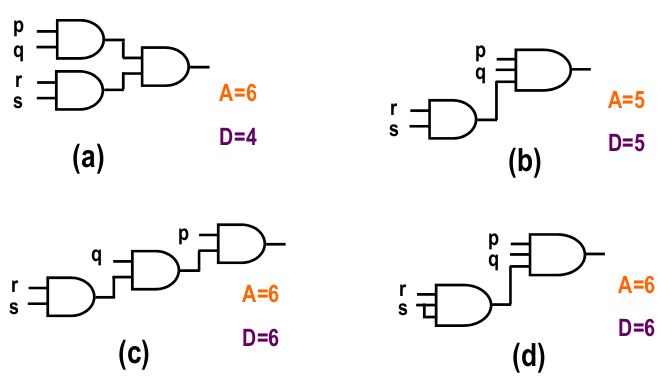
\includegraphics[width=\textwidth]{./Cap6/Images/Image1.png}
		\caption{Different Implementation}
		\label{fig:possImpl}
	\end{subfigure}
	\quad\quad
	\begin{subfigure}[b]{0.4\textwidth}
		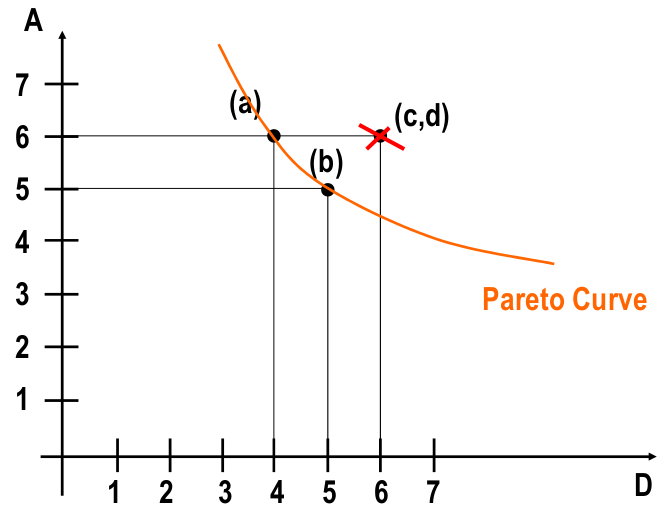
\includegraphics[width=\textwidth]{./Cap6/Images/Image2.png}
		\caption{Performance comparison}
		\label{fig:perform}
	\end{subfigure}
\end{figure}
In this case only (a) and (b) are part of pareto points, and they achieve different goal, in area or delay.

\subsection{Background and Definitions}
The \textbf{Boolean functions} we use in this case are:
\begin{itemize}
	\item \textit{Binary} Input and Output $ B = \{0, 1\} $ 
	\item \textit{Single} ( $ f : B^{n} \rightarrow B $ ) or\textit{ Multiple} (  $ f : B^{n} \rightarrow B^{m} $ ) output
	\item \textbf{Incompletely specified} so, functions \underline{with} don't care conditions ($ f: B^{n} = \{0, 1, *\} $)
\end{itemize}
\paragraph{Don't care condition}
The case in which we don't care about the value of a function, it's r\textit{related to the evirnonment} (input pattern that never occours or input patter for which some output is never observed),
\paragraph{ON-set}
Subset of the domain that make $ f = true $
\paragraph{OFF-set}
Subset of the domain that make $ f = false $
\paragraph{DC-set}
Subset of the domain for which we observe a \textit{don't care} value
\bigskip\\
For \textit{multiple output function}  ON, OFF and DC set is defined \textit{for each} component
\bigskip\\
We can give different representation that can be summarized into two categories: \textbf{visual} (Karnaugh Maps, Truth Table, Cubical Notation) or \textbf{computer oriented} (Matrices, BDDs) representations.
\begin{figure}[H]
	\centering
	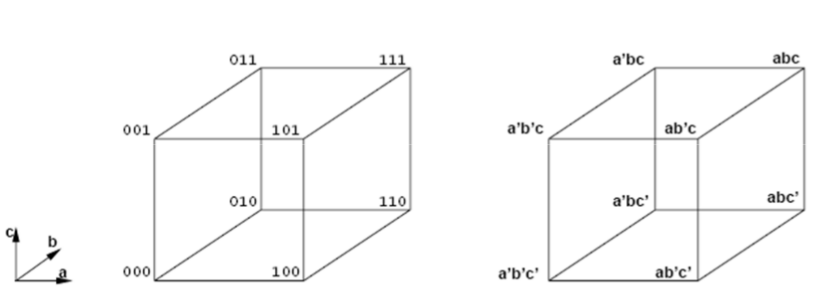
\includegraphics[width=0.6\textwidth]{./Cap6/Images/Image3.png}
	\caption{Cubical representation, in which each vertex of the cube is a minterm, can associate positional value. Example: $ ab'c \rightarrow 1_{a}0_{b}1_{c} $ \textit{(1 indicates true value)}}
	\label{fig:cubicalnotation}
\end{figure}
\paragraph{Definitions}
\begin{itemize}
	\item Boolean \textbf{variables} (\textit{Example: a, b, c, ...}) 
	\item Boolean \textbf{literals} are variables and their complement ( \textit{Example: a, a', b, b', ...})
	\item \textbf{Product or cube} is a product of literals (\textit{Example: ab'c, b'c, ...})
	\item A \textbf{Minterm} is product of \textit{all input variables} and implies a value for the function (usually 1)
	\item \textbf{Implicant} is a product (\textit{not mandatory to contain all the input variables}) that implies a value for the function (usually 1)
\end{itemize}
\paragraph{Tabular Representation}: define a truth ttable with the list of all minterm of a given function, and define a \textbf{cover} also called \textbf{implicant table} that is a list of all the implicant sufficient to define the function (\textit{Note}: implicant table is generally smaller in size than the truth table of the same function)

\begin{center}
	
	\begin{tabular}{|c|c|}
		\hline
		abc & xy \\ \hline
		000 & 00 \\ \hline
		001 & 10 \\ \hline
		010 & 00 \\ \hline
		011 & 11 \\ \hline
		100 & 00 \\ \hline
		101 & 01 \\ \hline
		110 & 11 \\ \hline
		111 & 11 \\ \hline 
	\end{tabular}
	\quad
	\quad
	\quad
	\quad
	\quad
	\quad
	\quad
	\begin{tabular}{|c|c|}
		\hline
		abc & xy \\ \hline
		001 & 10 \\ \hline
		*11 & 11 \\ \hline
		101 & 01 \\ \hline
		11* & 11 \\ \hline 
	\end{tabular}
	
	\bigskip
	Complete \textit{truth table} for $ x= ab + a'c $ and $ y = ab + bc+ ac $ (left side) and \textit{implicant table} (right side)
\end{center}
\paragraph{Logic Synthesis Problem} are related to the \textbf{implementation styles} (PLA macro-cells for \textit{two level circuits} and cell/array based for \textit{multi-level circuits}) and to the \textbf{operation mode} of the circuit (combinational, syncronous sequential or asyncronous sequential).

\subsection{Optimization for two-level circuits}
The reason why we invest so much time to the two level logic optimization are:

\begin{itemize}
	\item \textbf{Reduction} in the size of the representation
	\item \textbf{Direct implementation} of standard operating procedures (PLAs reduce size and delay).
	\item \textbf{implementation styles} based on Multi-Level nets
\end{itemize}

\subsubsection{Programmable Logic Arrays}
PLas are macro-cells with rectangular structure that implement any multi-output function. Their layout is generated by module generators and it's very popular in the '70/'80 but they are still used in some modern application, such as smart controllers, and in emerging technologies (Graphene, Crossbar Latch). They have some \textbf{advantages} as simplicity and predictable timing, but also the \textbf{disadvantages} of not much flexibility (with respect to cell based realization)
\paragraph{Graphene PLAs} are an open topic for researcher because there are interesting features of the graphene that allow us to recreate a complex function with a very low usage of gates (and so better performance and less area utilization)

\subsubsection{Approaches of Two-level Optimization}
Assuming that all implicants have the same cost, our goals are, the \textit{reduction of the number of implicants and literals}, infact implicants correspond to a PLA rows and literals to transistors.

\paragraph{Minimum cover} is the cover of a function with the \textit{minimum} number of implicants (\textbf{Global Optimum})

\paragraph{Minimal or irreduntant cover} is a cover that isn't a superset of another one (\textit{no implicant can be dropped}) and correspond to \textbf{local optimum}.

\paragraph{Minimal with respect to 1 implicant containment} cover in which no implicant is contained by another one (\textbf{weak local optimum})

Given this definition we can use \textit{exact methods} to compute \textit{\underline{minimum cover}} (often difficult/impossible for large function) or \textit{\underline{}} to compute \textit{\underline{minimal cover}}

\begin{itemize}
	\item \textbf{Exact Methods} are based on Quine's theorem (Quine-McCluskey, Petrick's methos, Espresso exact)
	\item \textbf{Heuristic Methods} MINI, PRESTO, ESPRESSO and so on.
\end{itemize}
Considering all possible implicant, we define some subset with some characteristics:
\begin{itemize}
	\item \textbf{Prime implicant}, implicant \textit{not} contained or covered by any other implicant
	\item \textbf{Prime cover} a cover in which \textit{all} implicants are prime
	\item \textbf{Essential Prime implicants} covers a minterm \textit{not} covered by any one else. They \textit{needs} to be included into the cover 
\end{itemize}
\subsubsection{Exact Logic Minimization}
The most used algorithms are based on \textit{Quine's theorem} that says:
\begin{center}
	\textit{There is a minimum cover that is prime}\\
\end{center}
and as consequence of this theorem we restrict our search of minimum cover only to prime implicants; for this reason the Quine-Based methods:
\begin{enumerate}
	\item Compute the prime implicants
	\item Determine the minimum cover
\end{enumerate} 
All the exact methods need the\textit{ primes table as starting point}, so that the optimization problem is reduced to a covering problem.\\
Considering a completely specified single-output functions, a \textbf{prime implicant table} is a binary-valued matrix $A$ whose columns are in one-to-one correspondence with the prime implicants of the function $f$ and whose rows are in one-to-one correspondence with its minterms.\\ 
A minimum cover is a minimum set of columns which covers all rows, or equivalently a minimum set of primes covering all minterms. Therefore the covering problem can be viewed as the problem of finding a binary vector $x$ representing a set of primes with minimum cardinality $|x|$ such that:
\begin{center}
	$Ax \geqslant \textbf{1}$
\end{center}
where \textbf{1} is the "unary vector" and as $x$ match he number of minterms and primes.

\paragraph{Example} given the function $ f= a'b'c' + a'b'c + ab'c + abc + abc' $

\begin{center}
	
	\begin{tabular}{|c|c|c|}
		\hline
		$\alpha$ & 00* & 1 \\ \hline
		$\beta$ & *01 & 1 \\ \hline
		$\gamma$ & 1*1 & 1 \\ \hline
		$\delta$ & 11* & 1 \\ \hline
	
	\end{tabular}
	\quad
	\quad
	\quad
	\quad
	\begin{tabular}{|c|c c c c|}
		\hline
		 {} & $\alpha$ & $\beta$ & $\gamma$ & $\delta$ \\ \hline
		 000 & 1 & 0 & 0 & 0 \\ \hline
		 001 & 1 & 1 & 0 & 0 \\ \hline
		 101 & 0 & 1 & 1 & 0 \\ \hline
		 111 & 0 & 0 & 1 & 1 \\ \hline
		 110 & 0 & 0 & 0 & 1 \\ \hline
		 
	\end{tabular}

	\bigskip
	
	\textit{Primes} to the left side, \textit{Prime table} to the right side
\end{center}

Then use the $x$ vector multiplied by $A$ to compute if all the implicant are covered, so:

\begin{center}
	
	\begin{tabular}{ c c }
	
		\begin{tabular}{|c c c c|}
			
			1 & 0 & 0 & 0 \\
			1 & 1 & 0 & 0 \\ 
			0 & 1 & 1 & 0 \\ 
			0 & 0 & 1 & 1 \\ 
			0 & 0 & 0 & 1 \\ 

			
		\end{tabular}
		
	\quad
	\quad
	
		\begin{tabular}{|c|}
			
			$x_{\alpha}$ \\
			$x_{\beta}$ \\
			$x_{\gamma}$ \\
			$x_{\delta}$ \\
			
		\end{tabular}
		
	\end{tabular}
	\bigskip
	
	Assigning to $x_{\alpha}, x_{\beta} ... $ value 1 only if it's considered part of the cover, then try to remove one of them from the cover and recompute if $Ax \geqslant \textbf{1}$, repeat this until find the \textit{minimum cover}.
\end{center}
\paragraph{Covering Problem} is a \underline{NP-hard problem} due to:
\begin{itemize}
	\item Columns - prime implicants (Up to $3^{n}/3$)
	\item Rows - minterms ($2^{n}$).
	\item Selection Boolean vector for primes $x$ and determine it such that $Ax \geqslant \textbf{1}$ 
	\item Select at the same time \textit{enough columns} to cover all rows and \textit{minimize the cardinality} of $x$.
\end{itemize}
\subsection{Quine-McCluskey}
The method involves two steps:
\begin{enumerate}
	\item Finding all prime implicants of the function.
	\item Use those prime implicants in a prime implicant chart to find the essential prime implicants of the function, as well as other prime implicants that are necessary to cover the function.
\end{enumerate} 
\paragraph{Example} Given the function $ f(x,y,z,v) = \Sigma m(1,4,5,6,7,9,11,14,15) $ so that the function will be equal to 1 for the values specified (1,4,5,6...), in the following step we attempt reduction and merge some minterms wher their \textit{mindistance  = 1}

\begin{center}
  
\begin{tabular}{ c c }
	
	\begin{tabular}{|c c c c|c c|}
		\hline
		x & y & z & v & res & val \\ \hline
		0 & 0 & 0 & 0 & 0 & {} \\ 
		0 & 0 & 0 & 1 & 1 & \textbf{m1} \\
		0 & 0 & 1 & 0 & 0 & {} \\
		0 & 0 & 1 & 1 & 0 & {} \\
		0 & 1 & 0 & 0 & 1 & \textbf{m4} \\
		0 & 1 & 0 & 1 & 1 & \textbf{m5} \\
		0 & 1 & 1 & 0 & 1 & \textbf{m6} \\
		0 & 1 & 1 & 1 & 1 & \textbf{m7} \\
		1 & 0 & 0 & 0 & 0 & {} \\
		1 & 0 & 0 & 1 & 1 & \textbf{m9} \\
		1 & 0 & 1 & 0 & 0 & {} \\
		1 & 0 & 1 & 1 & 1 & \textbf{m11} \\
		1 & 1 & 0 & 0 & 0 & {} \\
		1 & 1 & 0 & 1 & 0 & {} \\
		1 & 1 & 1 & 0 & 1 & \textbf{m15} \\	
		1 & 1 & 1 & 1 & 1 & \textbf{m14} \\ \hline
	\end{tabular}
	
	\quad
	\quad
	\quad
	
	\begin{tabular}{|c c c c c |c|}
		\hline
		{} & x & y & z & v & {} \\ \hline
		m1 & 0 & 0 & 0 & 1 & \checkmark \\ 
		m4 & 0 & 1 & 0 & 0 & \checkmark  \\
		m5 & 0 & 1 & 0 & 1 & \checkmark  \\
		m6 & 0 & 1 & 1 & 0 & \checkmark  \\
		m7 & 1 & 1 & 1 & 1 & \checkmark  \\
		m9 & 1 & 0 & 0 & 1 & \checkmark  \\
		m11 & 1 & 0 & 1 & 1 & \checkmark  \\
		m14 & 1 & 1 & 1 & 0 & \checkmark   \\
		m15 & 1 & 1 & 1 & 1 & \checkmark  \\ \hline
		
		
	\end{tabular}
	
	\quad
	\quad
	\quad
	
	\begin{tabular}{|c c c c c |c|}
		\hline
		
		{} & x & y & z & v & {} \\ \hline
		m1-m5 & 0 & * & 0 & 1 & \textbf{a} \\ 
		m1-m4 & * & 0 & 0 & 1 & \textbf{b}  \\
		m4-m5 & 0 & 1 & 0 & * & \checkmark  \\
		m4-m6 & 0 & 1 & * & 0 & \checkmark  \\
		m5-m7 & 0 & 1 & * & 1 & \checkmark  \\
		m6-m7 & 0 & 1 & 1 & * & \checkmark  \\
		m6-m14 & * & 1 & 1 & 0 & \checkmark  \\
		m7-m15 & * & 1 & 1 & 1 & \checkmark   \\
		m9-m11 & 1 & 0 & * & 1 & \textbf{c}  \\
		m11-m15 & 1 & 1 & 1 & * & \checkmark  \\ 
		m14-m15 & 1 & * & 1 & 1 & \textbf{d}  \\ \hline
		
	\end{tabular}
	
	\end{tabular}
	

	
	\begin{tabular}{|c c c c c |c|}
		\hline
		
		{} & x & y & z & v & {} \\ \hline
		m4-m5-m6-m7 & 0 & 1 & * & * & \textbf{e} \\ 
		m6-m7-m14-m15 & * & 1 & 1 & * & \textbf{f}  \\ \hline
		
	\end{tabular}

\end{center}
\bigskip
In this case \textbf{a, b, c, d, e, f} are implicant included into the cover because cannot be merged.\\
Now we have to identify the \textbf{essential prime implicants} and include it into the cover. To identify the essential we have to check if that implicant is the only one that cover \textit{a minterm}, in that case it's essential and has to be part of the cover.





\begin{center}
	
	\begin{tabular}{|c| c c c c c c|}
		\hline
		{} & a & b & c & d & \textbf{e} & \textbf{f} \\ \hline
		m1 & 1 & 1 & {} & {} & {} & {} \\
		m4 & {} & {} & {} & {} & \underline{\textbf{1}} & {} \\
		m5 & 1 & {} & {} & {} & 1 & {} \\
		m6 & {} & {} & {} & {} & 1 & 1 \\
		m7 & {} & {} & {} & {} & 1 & 1 \\
		m9 & {} & 1 & 1 & {} & {} & {} \\
		m11 & {} & {} & 1 & 1 & {} & {} \\
		m14 & {} & {} & {} & {} & {} & \underline{\textbf{1}} \\
		m15 & {} & {} & {} & 1 & {} & {} \\ \hline
		
	\end{tabular}
	
\bigskip
In this case \textit{e and f} are essential because they are the only that covers m4 (covered by e) and m14 (covered by f). Selecting these two implicans we have to consider all the minterms covered already by these. After that we can chose the prime implicants that are not essential. The only minterms that remain uncovered are: m1, m9, m11.

	\begin{tabular}{|c| c c c c |}
		\hline
		{} & a & \textbf{b} & \textbf{c} & d  \\ \hline
		m1 & 1 & 1 & {} & {} \\
		m9 & {} & 1 & 1 & {} \\
		m11 & {} & {} & 1 & 1 \\ \hline
	
	\end{tabular}
\bigskip

The final cover will be \textbf{ e, f, b, c } so that $f = yz + x'y + y'z'v + xy'v$ 

\end{center}

\subsection{Petrick's Method}


Petrick's method (also known as the \textit{branch-and-bound method}) is a technique for determining all minimum sum-of-products solutions from a prime implicant chart. Petrick's method is very tedious for large charts, but it is easy to implement on a computer. \\
It follows the same idea of Quine-McCluskey algorithm, reducing the table:

\begin{itemize}
	\item Iteratively identify essentials primes
	\item Save them in the cover
	\item Remove covered minterms
\end{itemize}

\paragraph{Petrick Algorithm} act in the following way:

\begin{itemize}
	\item Write covering clauses in \textit{product-of-sum form}
	\item Multiply out product-of-sum form into sum-of-product one (\textbf{this passage has an exponential cost})
	\item Select them the cube of minimum size
\end{itemize}

\paragraph{Example} Starting from \textit{Prime table} for the function $ f= a'b'c' + a'b'c + ab'c + abc + abc' $ :
\bigskip

\begin{center}
	\begin{tabular}{|c c|c c c c|}
	\hline
	{} & {} & $\alpha$ & $\beta$ & $\gamma$ & $\delta$ \\ \hline
	m0 & 000 & 1 & 0 & 0 & 0 \\ \hline
	m1 & 001 & 1 & 1 & 0 & 0 \\ \hline
	m5 & 101 & 0 & 1 & 1 & 0 \\ \hline
	m6 & 111 & 0 & 0 & 1 & 1 \\ \hline
	m7 & 110 & 0 & 0 & 0 & 1 \\ \hline
	
\end{tabular}
\end{center}

\begin{itemize}
	\item m0 is only covered by $\alpha$ $ \rightarrow $ m0 = $\alpha$
	\item m1 is covered by $\alpha$ and $\beta$ $ \rightarrow $ m1 = $\alpha$ + $\beta$
	\item m5 is covered by $\beta$ and $\gamma$ $ \rightarrow $ m5 = $\beta$ + $\gamma$
	\item m6 is covered by $\gamma$ and $\delta$ $ \rightarrow $ m6 = $\gamma$ + $\delta$
	\item m7 is only covered by $\delta$ $ \rightarrow $ m7 = $\delta$\\
\end{itemize}

So creating the product-of-sum form:\\
\begin{center}
	$(\alpha)(\alpha+\beta)(\beta+\gamma)(\gamma+\delta)(\delta) = 1$;\\
	$(\alpha+\alpha\beta)(\beta+\gamma)(\gamma\delta+\delta) = 1$;\\
	$(\alpha)(\beta+\gamma)(\delta) = 1$;\\
	$\alpha\beta\gamma + \alpha\gamma\delta = 1$;\\
\end{center}

in this case, to guarantee the cover of all minterms we have to solve the equation and have two different solution (both minumum) and we can chose to take $\alpha, \beta, \gamma$ or $\alpha, \gamma, \delta$


\subsection{Espresso-Exact}

The major improvements of the \textit{Espresso Exact} algorithm over the Quine-McCluskey algorithm consist of the construction of a \textbf{smaller reduced prime implicant table } and of the use of an efficient branch-and-bound algorithm for covering.\\

Espresso Exact partitions the prime implicants into three sets: essentials, partially redundunt and totally redundant. The \textbf{essentials} have the usual meaning, the \textbf{totally redundant} primes are those covered by the essentials and the don't care set, and the \textbf{partially redundant} set includes the remaining ones. The last set is the only one relevant to the covering phase, and it corresponds to the columns of the reduced implicant table. The rows of the reduced implicant table correspond to sets of minterms, rather than to single minterms as in the case of Quine-McCluskey's algorithm. Namely each row corresponds to all mintenns which are covered by the same subset of prime
implicants.
\bigskip 

\begin{center}
		\begin{tabular}{|c c|}
		\hline
		0000 & 1 \\
		0010 & 1 \\
		0100 & 1 \\
		0110 & 1 \\
		1000 & 1 \\
		1010 & 1 \\
		0101 & 1 \\
		0111 & 1 \\
		1001 & 1 \\
		1011 & 1 \\
		1101 & 1 \\
		\hline
	\end{tabular}
	\quad
	\quad
	$ \Leftrightarrow$
	\quad
	\quad
	\begin{tabular}{|c|c c|}
		\hline
		$ \alpha $ & 0**0 & 1 \\
		$ \beta $ & *0*0 & 1 \\
		$ \gamma $ & 01** & 1 \\
		$ \delta $ & 10** & 1 \\
		$ \epsilon $ & 1*01 & 1 \\
		$ \zeta $ & *101 & 1 \\
		\hline
	\end{tabular}
\end{center}

Prime implicants $ \gamma $ and $ \delta $ are essential, because they cover minterms 0111 and 1011 respectively, which are not covered by any other prime. The remaining primes are \textit{partially redundant}. The reduced prime implicant table is then:

\begin{center}
	\begin{tabular}{|c|c c c c|}
	\hline
	{} & $ \alpha $ & $ \beta $  & $ \epsilon $ & $ \zeta $ \\ \hline
	0000, 0010 & 1 & 1 & 0 & 0 \\
	1101 & 0 & 0 & 1 & 1 \\
	\hline
\end{tabular}

\end{center}

There are four different covers with minimum cardinality {$ \alpha, \gamma, \delta, \epsilon $}, {$ \beta,\gamma,\delta,\epsilon $} etc. that however include the essential prime implicants $ \delta, \gamma $ 

\begin{figure}[H]
	\centering
	\begin{subfigure}[b]{0.7\textwidth}
		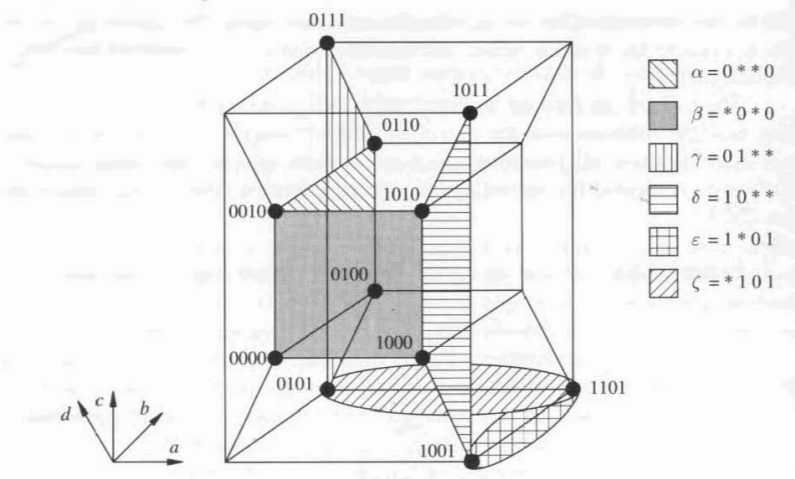
\includegraphics[width=\textwidth]{./Cap6/Images/Image4.png}
		\caption{Prime implicants}
		\label{fig:primeImpl}
	\end{subfigure}
	\quad
	\begin{subfigure}[b]{0.7\textwidth}
		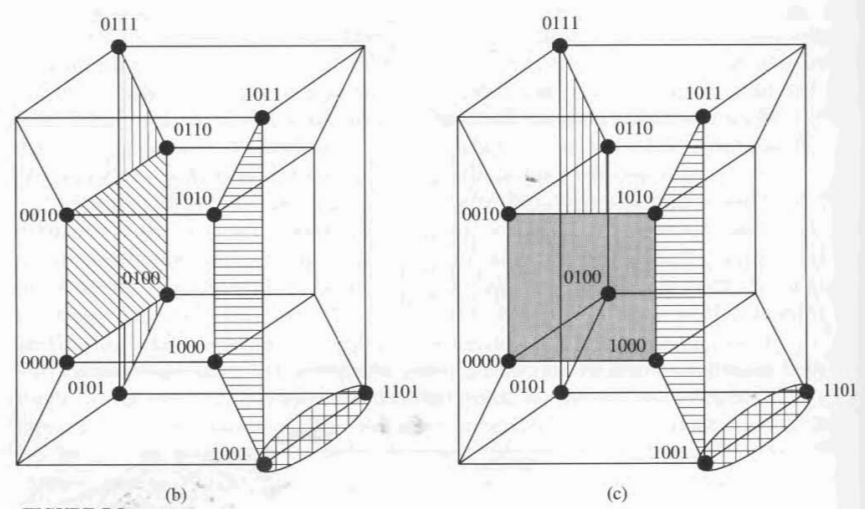
\includegraphics[width=\textwidth]{./Cap6/Images/Image5.png}
		\caption{Alternative Minimum Covers}
		\label{fig:altminim}
	\end{subfigure}
\end{figure}
\paragraph{Espresso-Exact two-level logic minimizer}
\begin{enumerate}
	\item select an arbitrary coloumn C
	\item using tabular methods and knowing that C will be part of the cover find the \textit{minimum} cover and evaluate cost function
	\item Assume than thet C will be not part of the cover and find the minimum
	\item Keep the best e reiterate
\end{enumerate}

\subsection{Heuristic Methods}

This methods were introduced to decrease the complexity of the exact algorithm that were the bottleneck of the optimization phase. The goal of this type of algorithm is to provide irredundant cover with \textit{reasonably small size} in a \textit{reasonable time}. What we are going to loose? The final cover will be a \textbf{minimal cover} and not minimum one. This type of methods for this reason find a \textit{local best} and not a global one infact the base of this algorithm are these steps:
\begin{enumerate}
	\item Start with an initial cover
	\item Search for feasible neighbours whose cost less.
	\item If found one, keep it and reiterate on that
\end{enumerate}

\begin{figure}[H]
	\centering
	\begin{subfigure}[b]{0.55\textwidth}
		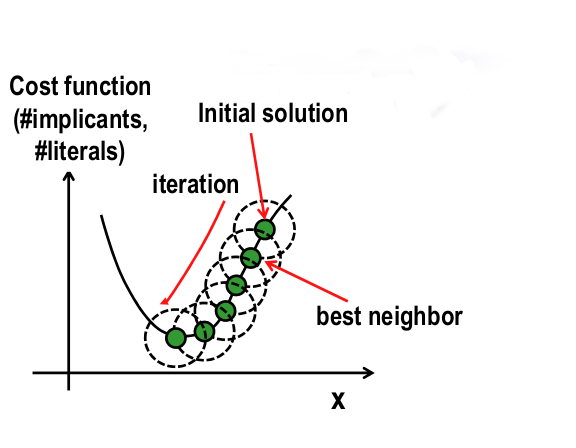
\includegraphics[width=\textwidth]{./Cap6/Images/Image6.png}
		\caption{Optimal case}
		\label{fig:heurbest}
	\end{subfigure}
	\quad
	\begin{subfigure}[b]{0.4\textwidth}
		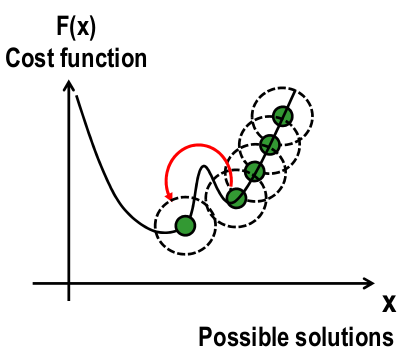
\includegraphics[width=\textwidth]{./Cap6/Images/Image7.png}
		\caption{The problem to have the search inside a limited scope}
		\label{fig:heurproblem}
	\end{subfigure}
\end{figure}

In this case is simple to understand that there are the main proble given to the local search that may stuck at a local minimum, so we need a mechanism to step out.\\

\paragraph{Heuristic optimization: Operators}

\begin{itemize}
	\item \textbf{Expand}, Make implicants prime (prime cover) and remove covered implicants.
	\item \textbf{Irredundant} make a prime cover irredundant (avoiding the minterms covered more than once)
	\item \textbf{Reduce} the size of each implicants preserving the cover, return a cover that is not prime
\end{itemize}

\paragraph{Expand operator}  makes a cover prime and minimal with respect to single-implicant containment. Implicants are processed one at a time. Each non-prime implicant is expanded to a prime(i.e., it is replaced by a prime implicant that contains it). Then, all other implicants covered by the expanded implicant are deleted.\\
\bigskip\\


An \textbf{example of Expansion} could be the following one:
\begin{itemize}
	\item Try to expand 0000
	\item raising to don't care one of the literals in this way, 0*00
	\item can be done only if 0000 and 0100 is both part of the cover
	\item if the previous condition is satisfied then drop 0100 to the cover and previous 0000 $ \rightarrow $ 0*00
\end{itemize}

\textit{Warning}: the previous operation has to be done for each literal of the considered minterm.

\paragraph{Irredundant operator} makes a cover irredundant. A minimal subset of implicants is selected such that no single implicant in that subset is covered by the remaining ones in that subset.
\bigskip\\
An \textbf{example of Irredundant operator} considering the cover ($ \alpha=0**0, \beta=*0*0, \gamma=01**, \delta=10**, \varepsilon= 1*01 $) could be the following one:
\begin{itemize}
	\item 00*0 contained into $ \alpha, \beta $
	\item 10*0 contained into $ \delta, \beta $
	\item 01*0 contained in $ \gamma, \alpha $
	\item in this case we can drop $ \alpha $ or $ \beta $ ( not $ \delta $ and $ \gamma $ because they are essential)
\end{itemize}

The previous cover is $ \alpha, \beta, \gamma, \delta, \varepsilon $ dropping $ \alpha $ the new cover will be $ \beta, \gamma, \delta, \varepsilon $ that is a minimal cover.

\paragraph{Reduce operator} transforms a cover into a non-prime cover with the same cardinality. Implicants are processed one at a time. The reduce operator attempts to replace each implicant with another that is contained in it, subject to the condition that
the reduced implicants, along with the remaining ones, still cover the function.
\bigskip\\

An \textbf{example of Reduce operator} considering the cover ($ \alpha=0**0, \beta=*0*0, \gamma=01**, \delta=10**, \varepsilon= 1*01 $) could be the following one:
\begin{itemize}
	\item reduce $ \alpha  = 0**0 $ to \textbf{nothing, drop the prime} (covered also by other).
	\item reduce $ \beta  = *0*0 $ to $ \beta'  = 00*0 $  
	\item reduce $ \varepsilon  = 1*01 $ to $ \varepsilon'  = 1101 $
\end{itemize}

So the new cover is {$ \beta', \gamma, \delta, \varepsilon'$} where we removed the don't care that bring to higher cost (so worst solution).

\subsubsection{Heuristic Espresso}

Exist different heuristics that differ in the type and sequence of operators applied. Espresso iteratively repeat this step:

\begin{enumerate}
	\item Expand + Irredundant (make the cover prime and irredundant, so \textit{find the best neighbor})
	\item Reduce (perturb the voer find some worst to \textit{step out of local minimum})  
	\item Reiterate until a small irredundant cover is obtained (possibly the global minimum)
\end{enumerate}

\paragraph{Espresso - Expand} starting from a minterm, try to delete one or more literals, in this case we have to \textbf{check the validity}, infact the expanded implicant needs to have \textit{void intersection withe the OFF-set}.

\begin{figure}[H]
	\centering
	\begin{subfigure}[b]{0.45\textwidth}
		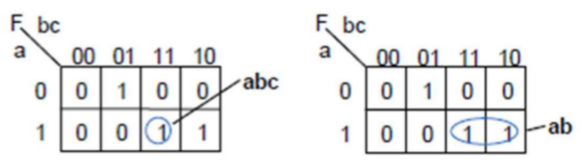
\includegraphics[width=\textwidth]{./Cap6/Images/Image8.png}
		\caption{Correct expansion}
		\label{fig:goodexpand}
	\end{subfigure}
	\quad
	\begin{subfigure}[b]{0.45\textwidth}
		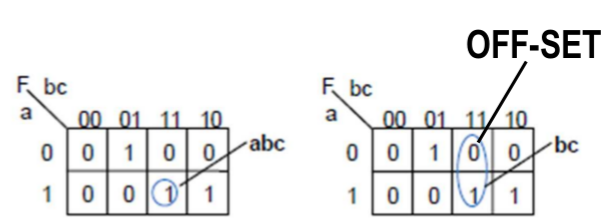
\includegraphics[width=\textwidth]{./Cap6/Images/Image9.png}
		\caption{Can't expand because the intersection with OFF-set is not void}
		\label{fig:badexpand}
	\end{subfigure}
\end{figure}

The \textbf{goal} is to expand non-prime implicant to prime with the \textit{latest} number of literals

\paragraph{Espresso - Irredundant} In this case the algorithm has to check for redundant implicants (redundant if all the minterms covered by that implicant are covered by other implicants contained into the cover)
\begin{figure}[H]
	\centering
	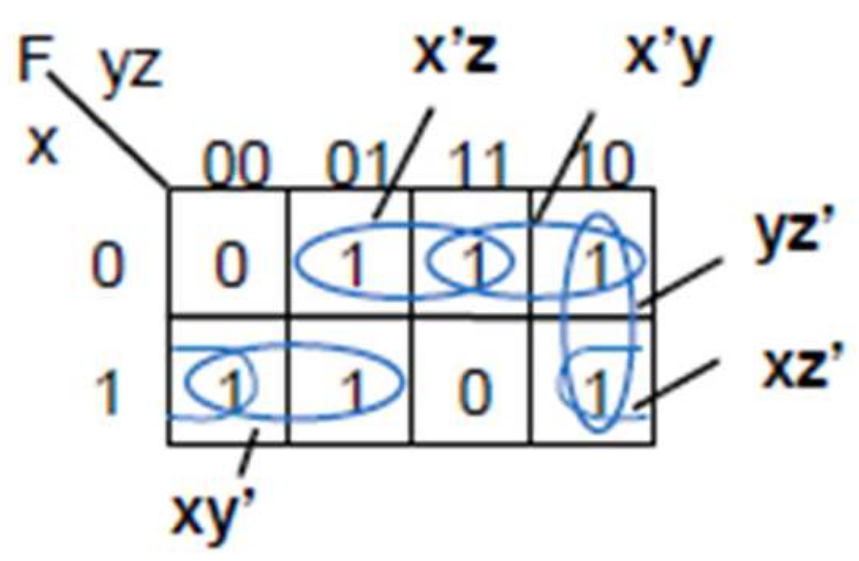
\includegraphics[width=0.4\textwidth]{./Cap6/Images/Image10.png}
	\caption{$yz'$ is redundant because $x'y$ and $xz'$ cover all minterms contained in $yz'$}
	\label{fig:checkredundant}
\end{figure}

\paragraph{Espresso - Reduce} In this case the algorithm starting from a prime implicant add one or more literlas and check for validity.
\begin{figure}[H]
	\centering
	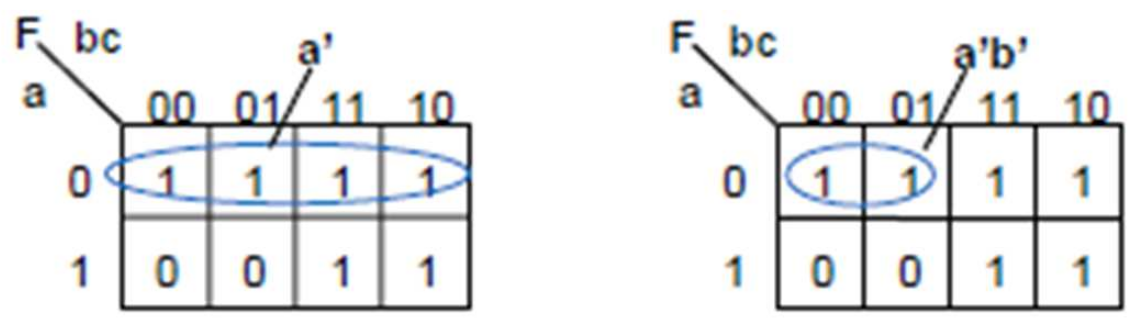
\includegraphics[width=0.6\textwidth]{./Cap6/Images/Image11.png}
	\caption{Reduce $a'$ adding $b'$ obtaining $a'b'$}
	\label{fig:reduceespresso}
\end{figure}

\textit{Why we want to do a reduction}? It brings to a \textit{worst} solution, it's true but, it help us to decrease the size of implicants such that \underline{next expansion} may lead to a better solution. We need this operation to step out te \textit{local minimum} (for this reason Reduce will never be the last operation).

\bigskip 

There are some additional concerns about Espresso, infact we have to:

\begin{itemize}
	\item check the validity of expansion
	\item decide the direction in which we move when make the expansion and reduction  
	\item how many literals drop (order of expansion)
\end{itemize}

\begin{figure}[H]
	\centering
	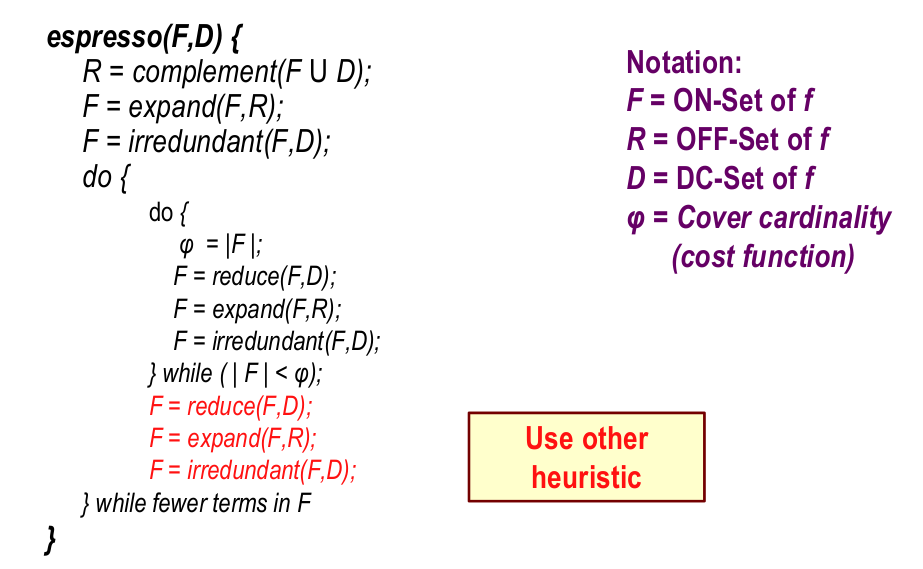
\includegraphics[width=0.7\textwidth]{./Cap6/Images/Image12.png}
	\caption{Espresso PseudoCode}
	\label{fig:espressopseudo}
\end{figure}

\subsection{Heuristic Optimization Tool}

Need this type of tools to check the validity of a cover using Containment and Complementation that use \textit{tautology} definition. There are some definition to prepare the background:

\begin{itemize}
	\item \textbf{Tautology}: check if a function is always true.
	\item \textbf{Containment}: check if a cube is contained in a cover, it's used in irreduntant operator (for example to find cubes contained in multiple primes).
	\item \textbf{Complementation}: Compute the complement of a function to find the OFF-set.\\  $OFFset = Complement( ONset + DCset )$ 
\end{itemize}

\paragraph{Other Definition} Given a function $f(x_{1}, x_{2},...x_{i},... x_{n})$:
\begin{itemize}
	\item \textbf{Cofactor of $f$ with respect to variable $x_{i}$ }: $f_{xi} = f(x_{1}, x_{2},...x_{i}=1,... x_{n})$
	\item \textbf{Cofactor of $f$ with respect to variable $x_{i}'$ }: $f_{xi'} = f(x_{1}, x_{2},...x_{i}=0,... x_{n})$
	\item \textbf{Boole's Expansion theorem}: $f(x_{1}, x_{2},...x_{i},... x_{n}) = x_{i}f_{xi}+x_{i}'f_{xi'} $
\end{itemize}

\paragraph{Example} Starting function $f = ab + bc + ac$:

\begin{itemize}
	\item $f_{a} = b+c$ because $b+c+bc = b+c$
	\item $f_{a'} = bc$
	\item Expansion: $f = af_{a} + a'f_{a'} = a(b+c) + a'bc$
\end{itemize}

\paragraph{Unateness(monotonicity)} Function $f(x_{1}, x_{2},...x_{i},... x_{n})$ is defined:

\begin{itemize}
	\item \textbf{Positive unate} in $x_{i}$ when $ f_{xi} \geq f_{xi'} $ 
	\item \textbf{Negative unate} in $x_{i}$ when $ f_{xi} \leq f_{xi'} $ 
\end{itemize}
A function is positive/negative unate when positive/negative unate in all its vaiables. In teh previous example $f_{a} = b+c$ and $f_{a'} = bc$:

\begin{center}
	\begin{tabular}{c | c | c |}
		
		$bc$ & \textbf{1} & \textbf{0} \\ \hline
		\textbf{1} & 1 & 0 \\ \hline 
		\textbf{0} & 0 & 0 \\ \hline  
		
		\hline
	\end{tabular}
	\quad
	\quad
	$ \leq $
	\quad
	\quad
	\begin{tabular}{ c | c | c |}
		$b + c$ & \textbf{1} & \textbf{0} \\ \hline
		\textbf{1} & 1 & 1 \\ \hline 
		\textbf{0} & 1 & 0 \\ \hline  
	\end{tabular}
\end{center}

\paragraph{Operators} Function $f(x_{1}, x_{2},...x_{i},... x_{n})$ is defined:

\begin{itemize}
	\item \textbf{Boolean difference} of $f$ with respect to variable $x_{i}$: $\delta f/\delta x_{i} \equiv f_{xi} \oplus f_{xi'}$ 
	\item \textbf{Consensus} of $f$ with respect to variable $x_{i}$: $C_{xi} \equiv f_{xi} \cdot f_{xi'}$ $\Rightarrow$ extract the part of the function independent by the variable under test.
	\item \textbf{Smoothing} of $f$ with respect to variable $x_{i}$: $S_{xi} \equiv f_{xi} + f_{xi'}$ $\Rightarrow$ function itself when you drop the variable.
\end{itemize}

\textbf{Tautology} plays an important role in all algorithms for logic optimization. Despite the intractability of the problem, the question if a function is a tautology can be answered efficiently using the recursive paradigm. To check it we have to define \textit{Matrix Representation}:

\begin{figure}[H]
	\centering
	\begin{subfigure}[b]{0.15\textwidth}
		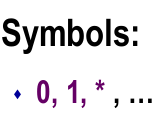
\includegraphics[width=\textwidth]{./Cap6/Images/Image13.png}
		\caption{Symbols}
		\label{fig:symbols}
	\end{subfigure}
	\quad
	\quad
	\quad
	\begin{subfigure}[b]{0.15\textwidth}
		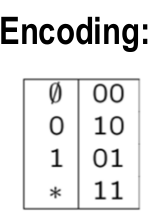
\includegraphics[width=\textwidth]{./Cap6/Images/Image14.png}
		\caption{Encoding}
		\label{fig:encoding}
	\end{subfigure}
	\quad
	\quad
	\quad
	\begin{subfigure}[b]{0.30\textwidth}
		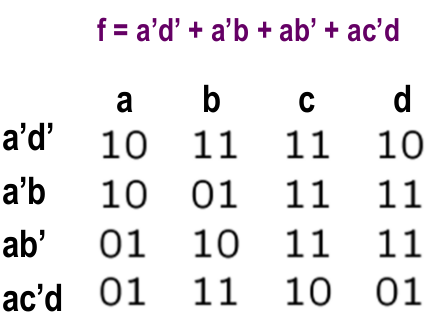
\includegraphics[width=\textwidth]{./Cap6/Images/Image15.png}
		\caption{Example of representation}
		\label{fig:represexample}
	\end{subfigure}
\end{figure}

We use this representation to better verify if a given cover, represent all the function. Infact, with the cube notation we follow this pseudocode to extract the cofactor for any variable:

\begin{center}
	$f_{xi} \rightarrow x_{i}$ (cube notation)\\
	for each row j of $f$ \\
	if($x_{i} \bigcap row_{j} \neq void$) \{ \\
		create \textbf{supercube} of $row_{j}$ with respect to $x_{i}$\}
		\bigskip\\
		where \textit{void representation is 00 }and \textbf{Supercube} is the rising to don't care of the variable $x_{i}$ and it's done with a \textbf{bitwise OR} 
\end{center}
\bigskip

We use this type of representation and this algorithm because we have some advantages:
\begin{itemize}
	\item \textbf{Binary values}, with two bits for each symbol and is more efficent than a char (8 bit minimum)
	\item We can apply binary operations for intersection (bitwise AND) and to calculate supercube (bitwise OR).
	\item Binary operation are really \textit{fast} and we could parallelize them.
\end{itemize}

So in this way we can calculate the cofactor and verify that f is a tautology, given that:

\begin{center}
\textit{a function $f$ is a tautology if and only if its cofactors with respect to any variable are a tautology.}
\end{center}

\paragraph{Example} given the function $f = a'b' + ab$:\\

\begin{center}
	
	\begin{tabular}{c  c}
		\begin{tabular}{c | c | c |}
			1 step & \textbf{a} & \textbf{b} \\ \hline
			\textbf{a'b'} & 10 & 10 \\ \hline 
			\textbf{ab} & 01 & 01 \\ \hline
		\end{tabular}
		\quad
		\quad
		\quad
		\quad
		\quad
		\quad
		\quad
		\begin{tabular}{ c | c | c |}
			{} & \textbf{a} & \textbf{b} \\ \hline
			\textbf{a} & 01 & 11 \\ \hline  
		\end{tabular}
	\end{tabular}
\end{center}

Then we can create the row of the table to verify the tautology in this way:\\

Take the value for a'b' in the cube notation table and do the \textbf{bitwise AND} with the row of a in the second table (cube notation of a):\\

\begin{center}
	\begin{tabular}{c  c}
		\begin{tabular}{c | c | c}
			10 & 10 & (cube notation a'b') \\ \hline
			01 & 11 & (cube notation of a)\\ \hline 
			00 & 10 & (bitwise AND) \\ \hline
			\textbf{void} & not void & (intersection)
		\end{tabular}
		\quad
		\quad
		\quad
		\quad
		\quad
		\quad
		\quad
		\begin{tabular}{c | c | c}
			01 & 01 & (cube notation ab) \\ \hline
			01 & 11 & (cube notation of a)\\ \hline 
			01 & 01 & (bitwise AND) \\ \hline
			not void & not void & (intersection)
		\end{tabular}
	\end{tabular}
\end{center}

	Only if all the intersection is not void all the intersection is not void, so in the first case the intersection is considered void, in the second one bot are not void, so, that row (bitwise AND) will contribuite to the final table:\\ 
	
\begin{center}
		\begin{tabular}{c | c | c}
		01 & 01 & (cube notation ab) \\ \hline
		10 & 00 & (\textit{complementary} of a)\\ \hline 
		\textbf{11} & \textbf{01} & (bitwise OR) \\
	\end{tabular}
\end{center}
	
Calculate the supercube in this way: $f_{a} = 11,01 = b$ (a corresponding to 11 is a don't care, b is positive in representation 01).\\

This is used in the \textbf{recursive paradigm}:

\begin{itemize}
	\item Expand about a variable
	\item Check if cofactors are a Tautology (if all cofactors are TRUE, then the function is a tautology otherwise the function is not)
\end{itemize}

\textit{When we stop?} There are these three \textbf{terminal cases}:
\\
\begin{itemize}
	\item The cover matrix has a row of all 1s(Tautology cube). \textbf{YES, TAUTOLOGY}
	\item The cover has a coloumn of all 0s, so a variable never takes a value. \textbf{NO TAUTOLOGY}
	\item The cover depends on only by one variable, and there is no coloumn of 0s in that field \textbf{YES, TAUTOLOGY}
\end{itemize}

\paragraph{FULL example of verification} Given a function $f= ab+ac+ab'c'+a'$:

\begin{center}
	\begin{tabular}{c || c | c | c}
	{} & a & b & c \\ \hline \hline
	ab & 01 & 01 & 11\\ \hline
	ac & 01 & 11 & 01\\ \hline 
	ab'c' & 01 & 10 & 10 \\ \hline
	a' & 10 & 11 & 11
	\end{tabular}
\end{center}

$f = af_{a} + a'f_{a'} \Leftrightarrow$ C(a) = 01 11 11 (a positive, b don't care, c don't care):\\

\begin{center}
	\begin{tabular}{c  c}
		\begin{tabular}{c c c c}
			01 & 01 & 11 & (cube notation ab) \\ 
			01 & 11 & 11 & (cube notation of a)\\ \hline 
			01 & 01 & 11 & (bitwise AND) \\ \hline
			not void & not void & not void & (intersection)
		\end{tabular}
		\quad
		\quad
		\quad
		\begin{tabular}{c  c  c c}
			01 & 01 & 11 & (cube notation ab) \\
			10 & 00 & 00 & (complementary of a)\\ \hline 
			\textbf{11} & \textbf{01} & \textbf{11} & (bitwise OR) \\ \hline
			\textbf{first} & \textbf{row} & \textbf{of} & \textbf{cofactor} \\
		\end{tabular}
	\end{tabular}
\end{center}

\begin{center}
	\begin{tabular}{c  c}
		\begin{tabular}{c c c c}
			01 & 11 & 01 & (cube notation ac) \\ 
			01 & 11 & 11 & (cube notation of a)\\ \hline 
			01 & 11 & 01 & (bitwise AND) \\ \hline
			not void & not void & not void & (intersection)
		\end{tabular}
		\quad
		\quad
		\quad
		\begin{tabular}{c  c  c c}
			01 & 11 & 01 & (cube notation ac) \\
			10 & 00 & 00 & (complementary of a)\\ \hline 
			\textbf{11} & \textbf{11} & \textbf{01} & (bitwise OR) \\ \hline
			\textbf{second} & \textbf{row} & \textbf{of} & \textbf{cofactor} \\
		\end{tabular}
	\end{tabular}
\end{center}

\begin{center}
	\begin{tabular}{c  c}
		\begin{tabular}{c  c  c c}
			01 & 10 & 10 & (cube notation ab'c') \\ 
			01 & 11 & 11 & (cube notation of a)\\ \hline 
			01 & 10 & 10 & (bitwise AND) \\ \hline
			not void & not void & not void & (intersection)
		\end{tabular}
		\quad
		\quad
		\quad
		\begin{tabular}{c  c  c c}
			01 & 10 & 10 & (cube notation ab'c') \\ 
			10 & 00 & 00 & (complementary of a)\\ \hline 
			\textbf{11} & \textbf{10} & \textbf{10} & (bitwise OR) \\ \hline
			\textbf{third} & \textbf{row} & \textbf{of} & \textbf{cofactor} \\
		\end{tabular}
	\end{tabular}
\end{center}

\begin{center}
		\begin{tabular}{c c c c}
			10 & 11 & 11 & (cube notation a') \\ 
			01 & 11 & 11 & (cube notation of a)\\ \hline 
			00 & 11 & 11 & (bitwise AND) \\ \hline
			\textbf{void} & not void & not void & (intersection)
		\end{tabular}
\end{center}

So the $f_{a}$ will be the following one:

\begin{center}
	\begin{tabular}{c | c | c}
		11 & 01 & 11 \\ \hline
		11 & 11 & 01 \\ \hline 
		11 & 10 & 10 \\ 
	\end{tabular}
\end{center}

C(a') = 10 11 11 (a negative, b don't care, c don't care):

\begin{center}
	\begin{tabular}{c c c c}
		01 & 01 & 11 & (cube notation ab) \\ 
		10 & 11 & 11 & (cube notation of a')\\ \hline 
		00 & 01 & 11 & (bitwise AND) \\ \hline
		\textbf{void} & not void & not void & (intersection)
	\end{tabular}
\end{center}

\begin{center}
	\begin{tabular}{c c c c}
		01 & 11 & 01 & (cube notation ac) \\ 
		10 & 11 & 11 & (cube notation of a')\\ \hline 
		00 & 11 & 01 & (bitwise AND) \\ \hline
		\textbf{void} & not void & not void & (intersection)
	\end{tabular}
\end{center}

\begin{center}
	\begin{tabular}{c c c c}
		01 & 10 & 10 & (cube notation ab'c') \\ 
		10 & 11 & 11 & (cube notation of a')\\ \hline 
		00 & 11 & 01 & (bitwise AND) \\ \hline
		\textbf{void} & not void & not void & (intersection)
	\end{tabular}
\end{center}

\begin{center}
	\begin{tabular}{c c}
		\begin{tabular}{c c c c}
			10 & 11 & 11 & (cube notation ab'c') \\ 
			10 & 11 & 11 & (cube notation of a')\\ \hline 
			10 & 11 & 11 & (bitwise AND) \\ \hline
			not void & not void & not void & (intersection)
		\end{tabular}
		\quad\quad
		\begin{tabular}{c  c  c c}
			10 & 11 & 11 & (cube notation a') \\ 
			01 & 00 & 00 & (complementary of a')\\ \hline 
			\textbf{11} & \textbf{11} & \textbf{11} & (bitwise OR) \\ \hline
			\textbf{first} & \textbf{row} & \textbf{of} & \textbf{cofactor} \\
		\end{tabular}
		
	\end{tabular}
\end{center}
 $f_{a'}$ = 11 11 11 and we can apply the first rule, so \textbf{it's a tautology}. \\
 
To $f_{a}$ we cannot apply any of the stopping rules, we have to continue with $f_{a|b}$ and $f_{a|b'}$, starting from $f_{a}$:

\begin{center}
		\begin{tabular}{c | c | c}
		a & b & c \\ \hline
		11 & 01 & 11 \\ \hline
		11 & 11 & 01 \\ \hline 
		11 & 10 & 10 \\
	\end{tabular}
\end{center}

b = 11 01 11

\begin{center}
	\begin{tabular}{c c}
		\begin{tabular}{c c c c}
			11 & 01 & 11 & (first row of $f_{a}$) \\ 
			11 & 01 & 11 & (cube notation of b)\\ \hline 
			11 & 01 & 11 & (bitwise AND) \\ \hline
			not void & not void & not void & (intersection)
		\end{tabular}
		\quad\quad
		\begin{tabular}{c  c  c c}
			11 & 01 & 11 & (first row of $f_{a}$) \\ 
			00 & 10 & 00 & (complementary of b)\\ \hline 
			\textbf{11} & \textbf{11} & \textbf{11} & (bitwise OR) \\ \hline
			\textbf{first} & \textbf{row} & \textbf{of} & \textbf{cofactor} \\
		\end{tabular}
	\end{tabular}
	
	\bigskip
	In this case we find a row of 1s, so for the first rule we can stop, \textbf{this is a tautology} $\Longrightarrow f_{a|b}$
\end{center}

Now we have to verify the $f_{a|b'}$: 

\begin{center}
	\begin{tabular}{c c c c}
		11 & 01 & 11 & (first row of $f_{a}$) \\ 
		11 & 10 & 11 & (cube notation of b')\\ \hline 
		11 & 00 & 11 & (bitwise AND) \\ \hline
		not void & \textbf{void} & not void & (intersection)
	\end{tabular}
\end{center}

\begin{center}
	\begin{tabular}{c c}
		\begin{tabular}{c c c c}
			11 & 11 & 01 & (second row of $f_{a}$) \\ 
			11 & 10 & 11 & (cube notation of b')\\ \hline 
			11 & 01 & 01 & (bitwise AND) \\ \hline
			not void & not void & not void & (intersection)
		\end{tabular}
		\quad\quad
		\begin{tabular}{c  c  c c}
			11 & 11 & 01 & (second row of $f_{a}$) \\ 
			00 & 01 & 00 & (complementary of b')\\ \hline 
			11 & 11 & 01 & (bitwise OR) \\ \hline
			\textbf{first} & \textbf{row} & \textbf{of} & \textbf{cofactor} \\
		\end{tabular}
	\end{tabular}
\end{center}

\begin{center}
	\begin{tabular}{c c}
		\begin{tabular}{c c c c}
			11 & 10 & 10 & (third row of $f_{a}$) \\ 
			11 & 10 & 11 & (cube notation of b')\\ \hline 
			11 & 10 & 10 & (bitwise AND) \\ \hline
			not void & not void & not void & (intersection)
		\end{tabular}
		\quad\quad
		\begin{tabular}{c  c  c c}
			11 & 10 & 10 & (third row of $f_{a}$) \\ 
			00 & 01 & 00 & (complementary of b')\\ \hline 
			11 & 11 & 10 & (bitwise OR) \\ \hline
			\textbf{second} & \textbf{row} & \textbf{of} & \textbf{cofactor} \\
		\end{tabular}
	\end{tabular}
\end{center}

So we obtain the table: 

\begin{center}
	\begin{tabular}{c c c}
		\hline
		11 & 11 & \textbf{01} \\ 
		11 & 11 & \textbf{10} \\ \hline 
		
	\end{tabular}
\end{center}

In this case we can apply the third rule, infact, we can note that $f_{a|b'}$ depend only on one variable. So $f_{a|b'}$ \textbf{is a tautology}.\\

We can conclude here infact, $f_{a}$, $f_{a|b}$ and $f_{a|b'}$ is a tautology $\Longrightarrow$ $f$ is a tautology.


\paragraph{Containment Theorem} A cover $F$ contains an implicant $\alpha$ if and only if $F_{\alpha}$ is a tautology. \textit{As consequence} containment can be verified by the tautology algorithm.


\paragraph{Example (Verify Containment)} Given a function $f= ab+ac+ab'c'+a'$, if we want to check covering of $bc$ start with the cofactor with respect to $bc$: 

\begin{center}
	\begin{tabular}{c | c | c}
		01 & 11 & 11 \\ \hline
		01 & 11 & 11 \\ \hline 
		10 & 11 & 11 \\ 
	\end{tabular}
\end{center}

In this case $f_{bc}$ depends only on $a$ and there is no column of 0s $\rightarrow$ \textbf{Tautology} $\rightarrow$ bc is contained by $f$

\paragraph{Complementation} Obtain $f'$ from $f$ is difficult for complex function but we can simlify it using this theorem: 

\begin{center}
	$f' = xf'_{x} + x'f'_{x'}$
\end{center}

So, we can follow this steps: 

\begin{itemize}
	\item Select a variable
	\item Compute co-factors
	\item Complement co-factors
\end{itemize}

Recur until one of this \textbf{termination rules} match:

\begin{itemize}
	\item Cover $F$ is void 
	\item The cover is a Tautology
	\item The cover $F$ consist only of one implicant
\end{itemize}


\paragraph{Example} $f = ab + ac + a'$, given the rule that $f' = xf'_{x} + x'f'_{x'}$, selecting the variable $a$:

\begin{center}
	\begin{tabular}{c || c | c | c}
		{} & a & b & c \\ \hline \hline
		ab & 01 & 01 & 11\\ \hline
		ac & 01 & 11 & 01\\ \hline 
		a' & 10 & 11 & 11
	\end{tabular}
\end{center}

and given C(a) = 01 11 11, $f_{a}$ will be:

\begin{center}
	\begin{tabular}{ c | c | c}
		11 & 01 & 11\\ \hline
		11 & 11 & 01\\ 
	\end{tabular}
\end{center}

In this case \textit{no rule match } so we must go with a new decomposition. Calculating  C(a') = 10 11 11, we find a row of 1 so, $f_{a'}$ = 11 11 11 $\rightarrow$ $f'_{a'}$ is \textbf{void}. $f' = af'_{a} + 0 $. In this case we have to compute $bf'_{ab} \cdot b'f'_{ab'} = f'_{a}$. Given C(b) = 11 01 11 we will end up with $f_{ab}$ :

\begin{center}
	\begin{tabular}{ c | c | c}
		11 & 11 & 11\\ \hline
		11 & 11 & 01\\ 
	\end{tabular}
\end{center}

That depend only by a variable so \textbf{it's a tautology}, for this reason $f'_{ab}$ is \textbf{void}. Given C(b') = 11 10 11 obtain $f_{ab'}$: 

\begin{center}
	\begin{tabular}{ c | c | c}
		11 & 11 & 01\\
	\end{tabular}
\end{center}

and its complement is \textit{11 11 10}. Now we have to reconstruct the complement intersecting (multipling) it with $b'$ and $a$ as given in the previous formulas $\rightarrow$ $f' = ab'c'$.

\begin{figure}[H]
	\centering
	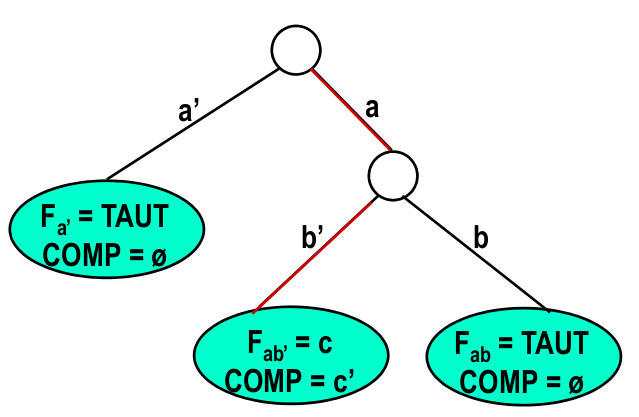
\includegraphics[width=0.45\textwidth]{./Cap6/Images/Image16.png}
	\caption{Example of computing complementation}
	\label{fig:compcomplement}
\end{figure}